
\documentclass{bredelebeamer}

\usepackage{kotex}
\usepackage{amsmath}
\usepackage{minted}

\DeclareMathOperator*{\minimize}{minimize}
\DeclareMathOperator*{\argmax}{arg\,max}
\DeclareMathOperator*{\argmin}{arg\,min} 
\setminted{fontsize=\footnotesize,baselinestretch=1}
\usemintedstyle{murphy}

\def\code#1{\texttt{#1}}

\title[Compiler Project Presentation]{컴파일러 프로젝트 발표}

\subtitle{}

\author{김규래, 박건}

\institute[Sogang University]
{
  서강대학교\\
}


\date{June 13 2019}
\subject{Design and Development of Compiler for C- Language}

\fontsize{11pt}{7.2}

%%%%%%%%%%%%%%%%%%%%%%%%%%%%%%%%%%%%%%%%%%%%%%%%%%%%%%%%%%%%%%%%%%%%%
\begin{document}

\begin{frame}
  \titlepage\
\end{frame}

\begin{frame}{세션에서 다룰 내용}
  \tableofcontents %[hideallsubsections]
  % You might wish to add the option [pausesections]
\end{frame}

\section{프로젝트 3 결과}
\subsection{Symbol Table 구현방법}
\begin{frame}{Symbol Table 구현방법}
	\begin{figure}
		\includegraphics[scale=0.3]{images/symtab.png}
	\end{figure}
\end{frame}

\begin{frame}{Symbol Table 구현방법}
	\begin{block}{Linked List of Hash Tables}
		\begin{itemize}
			\item Linked List의 각 노드가 해당 Scope의 Hash Table
			\item Scope에 들어갈 때 \code{st\_enter\_scope()} 함수로 Linked List에 노드 추가
			\item Scope가 종료될 때 \code{st\_exit\_scope()} 함수로 Linked List에서 노드 제거
			\item Semantic Analysis가 끝난 후 Symbol Table의 내용을 각 Scope별로 출력해야 하기 때문에 완전히 제거하지 않고, 따로 저장해 놓음. (\code{next} 필드)
		\end{itemize}
	\end{block}
\end{frame}

\begin{frame}[fragile]{Symbol Table 주요 코드}
	\begin{minted}
	[frame=lines,
	framesep=2mm,
	baselinestretch=0.7]{c}
/* The record in the bucket lists for
* each variable, including name, 
* assigned memory location, and
* the list of line numbers in which
* it appears in the source code
*/
typedef struct BucketListRec {
	const char* name;
	Record record;
	struct BucketListRec* next;
} * BucketList;

/* The local scope symbol table  */
typedef struct LocalSymbolTableRec {
	BucketList hashTable[SIZE];
	struct LocalSymbolTableRec* parent;
	struct LocalSymbolTableRec* next;
} * LocalSymbolTable;
	\end{minted}
\end{frame}

\begin{frame}[fragile]{Symbol Table 주요 코드}
	\begin{minted}
	[frame=lines,
	framesep=2mm,
	baselinestretch=0.7]{c}
void st_enter_scope(SymTable state)
{
    LocalSymbolTable table 
         = malloc(sizeof(struct LocalSymbolTableRec));
    for (int i = 0; i < SIZE; ++i) {
        table->hashTable[i] = NULL;
    }
    table->parent                 = state->currentScope;
    table->next                   = NULL;
    state->currentScope           = table;
    state->lastConstructed->next  = table;
    state->lastConstructed        = table;
}

void st_exit_scope(SymTable state)
{
    state->currentScope = state->currentScope->parent;
}
	\end{minted}
\end{frame}

\subsection{Semantic Analysis 구현방법}
\begin{frame}{Semantic Analysis 구현방법}
	\begin{itemize}
		\item 처음에는 복잡성을 줄이기 위해 Single Pass로 구현
		\item 그러나 나중에 수업시간에 배웠던 대로 Two Pass로 구현을 바꿈.
		\item 바꾸었더니 실행시간이 줄어듦.
	\end{itemize}
	
	\begin{figure}
		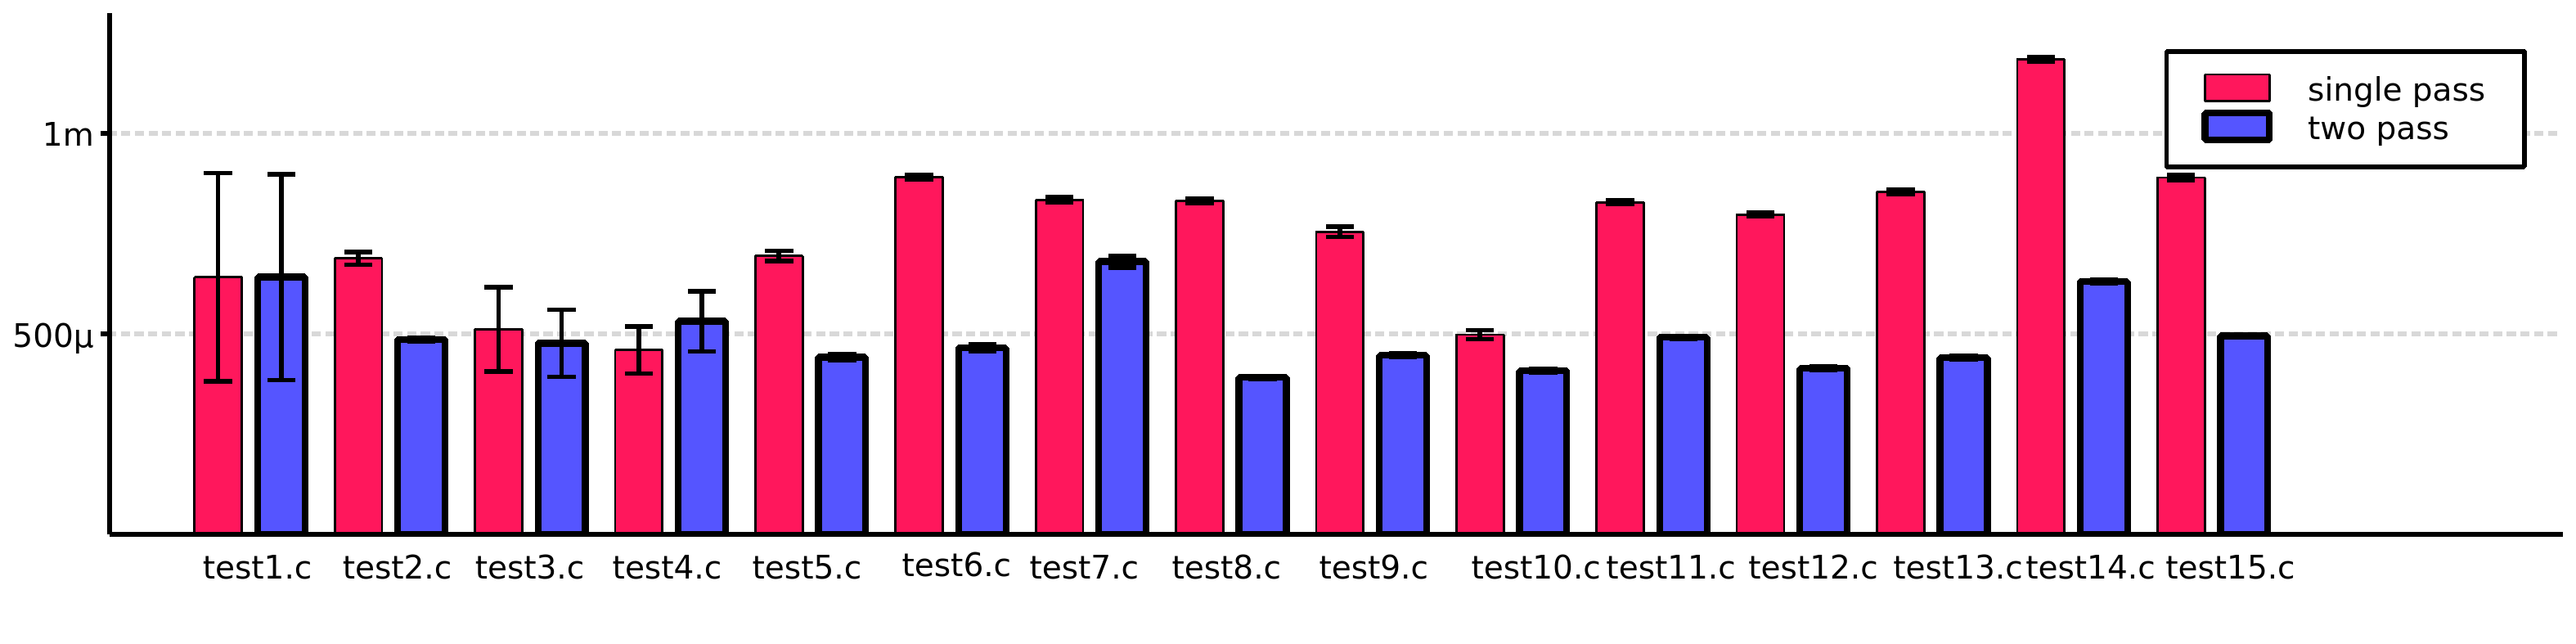
\includegraphics[scale=0.25]{figure/performance.png}
	\end{figure}
\end{frame}

\begin{frame}[fragile]{Location Counter 구현방법}
	\begin{minted}
	[frame=lines,
	framesep=2mm,
	baselinestretch=0.7]{c}
void main(void) {
    int a;
    {
        int b;
    }
    {
        int c;
    }
}
	\end{minted}
	\begin{itemize}
		\item 위와 같은 코드가 있을 때, \code{b}와 \code{c}는 같은 위치에 할당되어야 함.
		\item 
	\end{itemize}
\end{frame}

\subsection{테스트 방법}
\begin{frame}{테스트}
  \begin{tcolorbox}[tabvert,tabularx={X|Y}, boxrule=0.3pt]
    Version                      & Speedup \\\hline\hline
    Python                       & 1       \\
    C                            & 47      \\
    C parallelized               & 366     \\
    C parallelized \& memory opt & 6727    \\
    SIMD instructions            & 62806   \\\hline
  \end{tcolorbox}
  프레임워크/시스템/언어에 따른 성능의 장벽은 생각보다 높습니다.\footnote{Leiserson et al., \textit{There's Plenty of Room at The Top}, Under Review}
\end{frame}

\subsection{결과\textsl{}}
\begin{frame}{}
  \begin{block}{Latency 최소화}
    \begin{itemize}
    \item 각 연산을 수행하는데 걸리는 시간을 최소화
    \item CPU Clock 조정, 캐시 최적화, strength reduction
    \end{itemize}
  \end{block}

  \begin{exampleblock}{Throughput 최대화}
    \begin{itemize}
    \item 동일 시간에 처리하는 데이터의 양을 최대화
    \item 파이프라이닝, 병렬화
    \item 데이터의 양이 동일할 경우 전체적인 Latency 감소 효과
    \end{itemize}
  \end{exampleblock}
\end{frame}

\section{프로젝트 4 계획}
\begin{frame}{병렬화를 통한 Throughput 최대화}
  \begin{align*}
    \text{Throughput} = \text{sockets} \times
    \frac{\text{cores}}{\text{socket}} \times
    \frac{\text{cycles}}{\text{second}} \times
    \frac{\text{operations}}{\text{cycle}}
  \end{align*}

  \begin{block}{병렬화를 하는 다양한 수단들}
    \begin{itemize}
    \item CPU 에서 제공하는 SIMD instruction 을 사용
    \item Multithreading (Shared-memory parallelism)
    \item Distributed Computing (Distributed-memory parallelism)
    \item GPU, Xeon Phi 같은 병렬화에 특화된 하드웨어 사용
    \end{itemize}
  \end{block}
\end{frame}

\begin{frame}[fragile]{Results}
  \begin{itemize}
    \item Task Parallelism 을 사용할 경우 Loop Parallelism 에 비해서 더 높은 성능을 얻을 수가 있습니다.
    \item Loop Parallelism 에 비해서 파라미터 튜닝을 조금 더 거쳐야 합니다.
    \item 비동기 프로그래밍이라서 머리가 좀 더 아픕니다...
  \end{itemize}
\end{frame}

\begin{frame}[fragile]{Section}
  \begin{center}
    감사합니다
  \end{center}
\end{frame}
\end{document}

